\documentclass[aspectratio=64,8pt]{beamer}
\usepackage{tikz}

\usetikzlibrary{patterns}
\usetikzlibrary{overlay-beamer-styles}
\usepackage{txfonts}
\usepackage{soul}

\sethlcolor{yellow}
\newcommand{\mathhl}[1]{%
  \colorbox{yellow!90}{$\displaystyle #1$}%
}
%\usetikzlibrary{fit,calc,positioning}
\usepackage{pgfplots}
\usepackage{tcolorbox}
\usepackage{dsfont}
\usepackage{amsmath}
%\usepackage{amsfonts}
\usepackage{amssymb}
\usepackage{xcolor}
\usepackage{physics}
\usepackage{graphicx}
\usepackage{subcaption}
\usepackage{cancel}
%\usepackage{bbold}
\usepackage{multirow}
\usepackage{caption}
\usepackage{colortbl} 
\usepackage{qcircuit}
\usepackage{cancel}
\usepackage{proof}
\definecolor{bluClassico}{RGB}{15,76,129}
\usetikzlibrary{patterns}

\newcommand{\RNum}[1]{\uppercase\expandafter{\romannumeral #1\relax}}
\newcommand{\email}[1]{\def\insertemail{#1}}
\newcommand{\university}[1]{\def\insertuniversity{#1}}
\usetikzlibrary{overlay-beamer-styles}
\usetheme{Trento}  % Stored in /home/andrea/texmf/tex/latex/Trento
\addtobeamertemplate{navigation symbols}{}{%
    \usebeamerfont{footline}%
    \usebeamercolor[fg]{footline}%
    \hspace{1em}%
    \insertframenumber/\inserttotalframenumber
}

\title{G-steerability of Equivariant Neural Networks}
\subtitle{for (Hyper-)Nuclear Physics}
\author{\href{mailto:andrea.didonna@unitn.it}{Andrea Di Donna}}
\date{May 28, 2025}
\email{andrea.didonna@unitn.it}
\university{TIFPA - Trento University}

% Aggiunge ad ogni inizio di sezione un frame con l'indice della sola sezione corrente
\AtBeginSection[]{
  \begin{frame}{Sommario}
    \tableofcontents[currentsection]
  \end{frame}
}

\begin{document}
\frame{\titlepage}

%----------------------------------------------------

\begin{frame}{Equivariance formal Definition}
    \begin{itemize}
      \item We can interpret layers \(f(x)\) are \alert{functions} on feature fields (e.g. $\mathbb{R}^3$):
      \begin{equation}\nonumber
        f(x):\mathcal{F}_{\textrm{in}}\to\mathcal{F}_{\textrm{out}}
      \end{equation}
      and treat the subject with Group Theory formalism
      \item Let a group $G$ act on the input space $\mathcal{F}_{\mathrm{in}}$ via $g\rhd_{\textrm{in}} x$, and as $g\rhd_{\textrm{out}}f(x)$ on $\mathcal{F}_{\textrm{out}}$.
      \begin{columns}
        \begin{column}{0.25\linewidth}
        \begin{center}

          \textbf{Invariant Layer L}: 
          \\$L(g\rhd_{in}x)=L(x)$.
          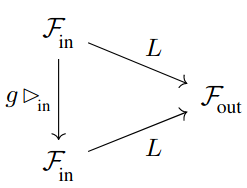
\includegraphics[width=1\textwidth]{Immagini/Invariance.png}
        \end{center}          
        \end{column}

        \begin{column}{0.3\linewidth}
          \begin{center}
            \textbf{Equivariant Layer $\mathcal{T}$}: \\$\mathcal{T}(g\rhd_{\textrm{in}}x)=g\rhd_{\textrm{out}}\mathcal{T}(x)$.     
            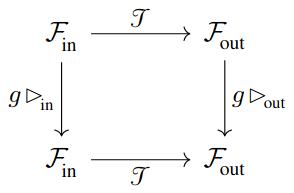
\includegraphics[width=1\textwidth]{Immagini/Commutativity_Equivariance.png}
          \end{center}          
        \end{column}
      \end{columns}
      
      \begin{tcolorbox}[title=\textbf{What's the role of equivariance in Physics?},colback=blue!5!white]
          \vspace{-10pt}
        \begin{columns}

            \begin{column}{0.28\linewidth}
              {\small 
              \begin{equation}\nonumber
                \Psi(\vec{r}-\vec{x}) = e^{-i\hat{p}\cdot\vec{x}}\Psi(\vec{r})
              \end{equation}
              }
            \end{column}

            \begin{column}{0.72\linewidth}
              {\small 
              \begin{equation}\nonumber
               P_{ij}\mathcal{A}(\dots\otimes \psi_{\alpha}(\vec{x}_i)\otimes\dots\otimes\psi_{\beta}(\vec{x}_j) \otimes \dots) = - \mathcal{A}(\dots\otimes\psi_{\alpha}(\vec{x}_i)\otimes\dots\otimes\psi_{\beta}(\vec{x}_j)\otimes\dots)
              \end{equation}
              }
            \end{column}
          \end{columns}
          \begin{columns}
            %\begin{column}{0.28\linewidth}
            %  {\small 
            %  \begin{equation}\nonumber
            %    \Psi(x+dx) = e^{i\vec{p}\cdot\vec{x}\Psi}
            %  \end{equation}
            %  }
            %\end{column}

            \begin{column}{1\linewidth}
              {\small 
              \vspace{5pt}
              \begin{equation}\nonumber
                  \pi^a(x) \longmapsto U_{\boldsymbol{\theta}}(\pi^a(x))=D^{ba}(U_{\boldsymbol{\theta}})\,\pi^a(x),
                  \qquad U=\exp\bigl(i\sum \boldsymbol{\theta} \cdot \boldsymbol{\tau}/2\bigr)
                \end{equation}
              }
            \end{column}
          \end{columns}

      \end{tcolorbox}
      \item     Composition of equivariant layers are equivariant Neural Networks

    \end{itemize}
\end{frame}




\begin{frame}{Intertwiners and Equivariant Layers}
  \vspace{-25pt}
  \begin{tcolorbox}[title=\textbf{Intertwiner (Weiler \& Cohen 2019)},colback=blue!5!white]

  A linear map $W$ between representations $\rho_{\text{in}},\rho_{\text{out}}$ of $G$ is an \alert{intertwiner} if
  \[
    (\star) \qquad W\,\rho_{\text{in}}(g)=\rho_{\text{out}}(g)\,W,
      \qquad\forall g\in G .
  \]
  In terms of matrix representations, this just means that there exists \alert{a change of basis} (invertible intertwiner) $W$ such that the representations are similar as matrices:
  \[
    \rho_{\text{in}}(g)=W^{-1}\,\rho_{\text{out}}(g)\,W,
    \qquad\forall g\in G .
  \]
  \end{tcolorbox}

  \vspace{0.5em}
  \begin{center}
    \textbf{Symmetric Group $S_n$: }$G=\mathsf S_n$ acts by permuting the indices of a set $X=\{x_1,\dots,x_n\}$.      \
  \end{center}

  \begin{columns}
    \begin{column}{0.5\textwidth}
      \textbf{Antisymmetrizer -- $S_n$ Antisymm Equiv.}\\
      \vspace{-10pt}
      $$
      \boxed{\;
      \mathcal{A}\,P_h=\operatorname{sgn}(h)\, \mathcal{A}
      \; \quad  \mathcal{A} \;=\; \frac{1}{n!}\;\sum_{g\in S_n}\!\operatorname{sgn}(g)\,P_g
     }
      $$
    \end{column}
    \begin{column}{0.5\textwidth}
      \textbf{Deep Sets -- $S_n$ Permutation Invariance.}\\
      \vspace{-10pt}
    \[
      \boxed{\;
      W_{\text{sum}}P_h\;=\;\mathds{1}W_{\text{sum}} \quad  \Phi(X)= \rho\Bigl(\sum_{i=1}^{n} h(x_i)\Bigr),
      }
      \]
    \end{column}
  \end{columns}


\end{frame}



\begin{frame}{Group Convolution}
    \textbf{Due paradigmi di convoluzione \(\;\Rightarrow\;\) un unico obiettivo}

  \begin{enumerate}

      \item \textbf{Group Convolution}\\[2pt]
          \[
            (k\star_G f)(g)
            \;=\;
            \int_G k(g^{-1}h)\,f(h)\,dh,
            \qquad
            k,f : G \to V.
          \]
          \(\star_G\) è automaticamente equivariante \(\bigl[(L_{g'}k)\star_G(L_{g'}f)=L_{g'}(k\star_G f)\bigr]\),
          ma l’integrale su \(SO(3)\) è oneroso.
  \end{enumerate}
       \textbf{Osservazione — Cohen et al. (2018)}\\[2pt]
      La doppia integrazione richiesta da \(\star_G\) su \(SO(3)\)
      (dominio e kernel) è impraticabile in una rete deep;  
      meglio vincolare analiticamente il kernel in modo steerable
      e integrare solo sullo \emph{dominio fisico}.
\end{frame}

\begin{frame}{G-steerable convolution}
\begin{enumerate}\setcounter{enumi}{1}
  \item \textbf{G-steerable Convolution (spazio fisico)}\\[2pt]
  \centering
  \boxed{ (k\star f)(\mathbf x)
           \;=\;
           \int_{\mathbb R^3} K(\mathbf x-\mathbf y)\,f(\mathbf y)\,d\mathbf y,
           \quad
           K(R\hat{\mathbf r}) = R\,K(\hat{\mathbf r})\,R^{\!\top}.
        }

        L’equivarianza è \emph{impacchettata} nella forma chiusa di \(K\).

  \vspace{4pt}

\end{enumerate}
        \begin{itemize}
              \item \emph{Group convolution}\(\star_G\): integra sia sul dominio che sul gruppo.
              \item \emph{G-steerable convolution}: integra solo sul dominio; la parte angolare è incorporata 
              analiticamente nel kernel.
              \item \textbf{Equivalenza teorica}: un kernel G-steerable che soddisfa \(K(R\hat r)=R K(\hat r)R^{\!\top}\) 
              implementa la stessa trasformazione indotta da \(\star_G\), ma con costo computazionale ridotto.
        \end{itemize}
\end{frame}

\begin{frame}[fragile]{Kernel Sferico e Steerability}
\[
  K(\mathbf r)
  \;=\;
  \sum_{J=0}^{2} \varphi_J(r)
  \sum_{m=-J}^{J}
  Y_{Jm}\!\bigl(\hat{\mathbf r}\bigr)\;
  Q_{Jm}^{\ell,\ell_in},
  \qquad
  \hat{\mathbf r}=\frac{\mathbf r}{\lVert\mathbf r\rVert}.
\]

\begin{itemize}
  \item \textbf{Separazione radiale/angolare}:\\[2pt]
        \(\varphi_J(r)\) è la parte \emph{learnable} (solo raggio),  
        \(Y_{Jm}(\hat{\mathbf r})\) sono basi fisse sul \(S^2\).
  \item \textbf{Steerability}:\\[2pt]
        \(Y_{Jm}\bigl(R\,\hat{\mathbf r}\bigr)
        =\displaystyle\sum_{m'=-J}^{J} D^{J}_{m'm}(R)\,Y_{Jm'}(\hat{\mathbf r})\)\\
        \(\Longrightarrow\;
        K(R\hat{\mathbf r}) = R\,K(\hat{\mathbf r})\,R^{\!\top}\).
  \item \(Q_{Jm}\) sono i coefficienti di Clebsch–Gordan che accoppiano
        \(\ell_{\text{in}}=\ell_{\text{out}}=1\) 
        ai tre canali angolari \(J=0,1,2\).
\end{itemize}

\[
  \boxed{\;K\star f \;\text{è automaticamente }SO(3)\text{-equivariante}\;}
\]
\end{frame}


\begin{frame}[fragile]{Equivalenza dei kernel (TFN\,$\leftrightarrow$\,contratto)}
\[
\underbrace{\sum_{\scriptstyle J=0}^{2}\!\varphi_J(r)\sum_{m=-J}^{J}Y_{Jm}(\hat{\mathbf r})\,Q^{(J)}_{m}}_{\text{kernel TFN per }\ell_{\text{in}}=\ell_{\text{out}}=1}
\;=\;
\underbrace{a(r)I\; +\; b(r)[\hat r]_\times\; +\; c(r)Q(\hat r)}_{\text{kernel contratto}}
\]
\vspace{0.5em}
\begin{itemize}
  \item La somma sui coefficienti di Clebsch--Gordan $Q^{(J)}_{m}$ \emph{contratta} gli indici $m$.
  \item Produce tre tensori cartesiani ortogonali: $I$, $[\hat r]_\times$, $Q(\hat r)$.
  \item Le funzioni radiali corrispondono: $a\!\propto\!\varphi_0$, $b\!\propto\!\varphi_1$, $c\!\propto\!\varphi_2$.
  \item Stessa legge di trasformazione $\Rightarrow$ stessa equivarianza.
\end{itemize}
\vspace{-0.5em}
\[
\boxed{\text{Kernel TFN}\;\equiv\;\text{Kernel contratto (nostro)}}
\]
\end{frame}



\begin{frame}{Il nostro kernel equivariante}
\begin{equation}\nonumber
  K(\mathbf r)=a(r)I\; +\; b(r)[\hat{\mathbf r}]_\times\; +\; c(r)\,Q(\hat{\mathbf r}),
  \qquad \hat{\mathbf r}=\frac{\mathbf r}{\lVert\mathbf r\rVert}.
\end{equation}

\hspace{-20pt}
\begin{equation} \nonumber
    \renewcommand{\arraystretch}{1.2}
I=\begin{pmatrix}1&0&0\\0&1&0\\0&0&1\end{pmatrix}, \quad
[\hat{\mathbf r}]_\times=\begin{pmatrix}0&-\hat r_z&\hat r_y\\\hat r_z&0&-\hat r_x\\-\hat r_y&\hat r_x&0\end{pmatrix}, \quad
Q(\hat{\mathbf r})=3\begin{pmatrix}
 \hat r_x^2 & \hat r_x\hat r_y & \hat r_x\hat r_z\\
 \hat r_y\hat r_x & \hat r_y^2 & \hat r_y\hat r_z\\
 \hat r_z\hat r_x & \hat r_z\hat r_y & \hat r_z^2
\end{pmatrix}-I.
\end{equation}

\vspace{0.5em}
\begin{itemize}
  \item Caso particolare \(\ell_{\text{in}}=\ell_{\text{out}}=1\) del kernel TFN.
  \item Tre canali angolari \(J=0,1,2\) \(\Rightarrow\) tre funzioni radiali \(a,b,c\).
  \item Equivarianza garantita da \(K(R\hat r)=R\,K(\hat r)R^{\!\top}\,\,\forall R\in SO(3).\)
\end{itemize}
\end{frame}





\begin{frame}{ \((\ell_\text{out}=1) \) proof of \([r]_\times \) equivariance}
\vspace{-10pt}
    \begin{lemma}{Equivarianza del termine \(b(r)\,[\hat r]_\times f \)}
Sia  \(R\in SO(3) \),  \(\hat r=\tfrac{r}{\mid r \mid} \) e \([\hat r]_{\times,ij}=\varepsilon_{ijk}\,\hat r_k \).
Definiamo  \(g=b(\mid r \mid)\,[\hat r]_\times f\in\mathbb R^3 \). Allora, per  \(f' = R f \) e  \(\hat r' = R \hat r \),
\[
g' \;:=\; b(\mid r \mid)\,[\hat r']_\times f' \;=\; R\,g,
\]
cio\`e \(g \) trasforma come un vettore (\(\ell=1 \)).
\end{lemma}
\vspace{-10pt}
\begin{proof}
Poich\'e  \(b(\mid r\mid ) \) dipende solo da  \(\mid r\mid \), \`e invariante per rotazioni. In indici,
\[
([\hat r']_\times)_{ij} \;=\; \varepsilon_{ijk}\,\hat r'_k
\;=\; \varepsilon_{ijk}\,R_{k\ell}\,\hat r_\ell.
\]
Usiamo l'invarianza del simbolo di Levi--Civita sotto rotazioni proprie,
\[
R_{ip}R_{jq}R_{kr}\,\varepsilon_{pqr} \;=\; \varepsilon_{ijk},
\]
che \`e equivalente a  \([R v]_\times = R [v]_\times R^\top \). Allora
\[
([\hat r']_\times)_{ij}
= R_{ip}R_{jq}\,\varepsilon_{pq\ell}\,\hat r_\ell
= (R[\hat r]_\times R^\top)_{ij}.
\]
Quindi
\[
g'_i = b(\mid r \mid)\,([\hat r']_\times)_{ij} f'_j
= b(\mid r \mid)\,(R[\hat r]_\times R^\top)_{ij}\,R_{jm} f_m
= b(\mid r \mid)\,R_{ip}\,[\hat r]_{\times,pm}\,f_m
= (R g)_i,
\]
dove abbiamo usato \(R^\top R = I\). Pertanto \(g' = R g\).
\end{proof}

\end{frame}


\begin{frame}{$(\ell_{out}=1)$ proof of $Q(\hat{r})$ equivariance }
\begin{lemma}[Equivarianza del termine $c(r)\,Q(\hat r)\,f$]
Sia $Q_{ij}(\hat r)=3\,\hat r_i \hat r_j - \delta_{ij}$. Definiamo $h=c(\mid r \mid)\,Q(\hat r)\,f\in\mathbb R^3$.
Allora, per $f' = R f$ e $\hat r' = R \hat r$,
\[
h' \;:=\; c(\mid r \mid)\,Q(\hat r')\,f' \;=\; R\,h,
\]
cio\`e $h$ trasforma come un vettore ($\ell=1$).
\end{lemma}

\begin{proof}
Poich\'e $c(\mid r \mid)$ dipende solo da $\mid r \mid$, \`e invariante per rotazioni. In indici,
\[
Q_{ij}(\hat r') = 3\,\hat r'_i \hat r'_j - \delta_{ij}
= 3\,R_{ik}\hat r_k\, R_{j\ell}\hat r_\ell - \delta_{ij}
= R_{ik} R_{j\ell}\,(3\,\hat r_k \hat r_\ell - \delta_{k\ell})
= (R Q(\hat r) R^\top)_{ij}.
\]
Quindi
\begin{align}\nonumber
h'_i
&= c(\mid r \mid)\,Q_{ij}(\hat r')\,f'_j
= c(\mid r \mid)\,(R Q R^\top)_{ij}\,R_{jm} f_m
= c(\mid r \mid)\,R_{ik}\,Q_{k\ell}\,(\underbrace{R^\top R}_{I})_{\ell m}\,f_m
\\ &=R_{ik}\,(Q f)_k
= (R h)_i.\nonumber
\end{align}

Ne segue $h' = R h$.
\end{proof}

    
\end{frame}
\begin{frame}{Other implementations}
\begin{table}[h]\hspace{-20pt}
\renewcommand{\arraystretch}{1.25}
\begin{tabular}{c|l|l|l}
\hline
$\ell_{\text{out}}$ &
$K(\hat{\mathbf r},r)$ (forma del kernel) &
Azione su $f_b \in \mathbb{R}^3$ &
\shortstack[l]{Canali irred.\ usati \\$(\ell_\text{in}^{=1} \otimes \ell_\text{ker} \to \ell_{\text{out}})$} 
\\
\hline
$0$ &
$K_b(\hat{\mathbf r},r)=\alpha(r)\,\hat r_b\;(\ell_f=1)$ &
$y \;=\; K_b f_b \;=\; \alpha(r)\,\hat{\mathbf r}\!\cdot\!\mathbf f$ &
$1\otimes 1 \to 0$ \quad $(\ell_f=1)$
\\\hline
$1$ &
\begin{equation}
    \nonumber
    \begin{aligned}
        &a(r)\,\delta_{ab}\;(\ell_f=0)\;+\\
        K_{ab}(\hat{\mathbf r},r)=&b(r)\,\epsilon_{abc}\,\hat r_c\;(\ell_f=1)\;+\\
        &c(r)\,Q_{ab}(\hat{\mathbf r})\;(\ell_f=2)
    \end{aligned}
\end{equation}
&
$g_a \;=\; K_{ab}\,f_b$ &
\begin{equation}
    \nonumber
    \begin{aligned}
        &1\otimes 0 \to 1\\
        &1\otimes 1 \to 1\\
        &1\otimes 2 \to 1
    \end{aligned}
\end{equation}

\\ \hline
$2$ &
\begin{equation}
    \nonumber
    \begin{aligned}
K_{ab,c}(\hat{\mathbf r},r)= &\alpha(r)\,\mathrm{ST}\!\big(\hat r_a \delta_{bc} + \hat r_b \delta_{ac}\big)\;(\ell_f=1)\;+\\
&\;
\beta(r)\,\mathrm{ST}\!\big(Q_{ab}(\hat{\mathbf r})\,\hat r_c\big)\;(\ell_f=2)
\end{aligned}
\end{equation}
&
$T_{ab} \;=\; K_{ab,c}\,f_c$ &
\begin{aligned}
&1\otimes 1 \to 2\\
&1\otimes 2 \to 2
\end{aligned}
\\
\hline
\end{tabular}
\caption{Kernel equivariante per $\ell_{\text{in}}=1 \to \ell_{\text{out}}\in\{0,1,2\}$.
Si usa $Q_{ab}(\hat{\mathbf r}) = 3\,\hat r_a \hat r_b - \delta_{ab}$ e
$\mathrm{ST}(X_{ab}) = \tfrac{1}{2}(X_{ab}+X_{ba}) - \tfrac{1}{3}\delta_{ab}\,X_{cc}$.
Le funzioni radiali $\alpha,\beta,a,b,c$ dipendono da $r=\|\mathbf r\|$. I tag $(\ell_f=\cdot)$
indicano il grado del pezzo angolare del kernel.}
\label{tab:kernels-l1-irreps}
\end{table}
\end{frame}



\begin{frame}[fragile]{Dal continuo al discreto \;(\(\mathbb R^3\) campionato)}
\[
( K\!\star f )(\mathbf x)
\;=\;\int_{\mathbb R^3}\!K(\mathbf x-\mathbf y)\,f(\mathbf y)\,d\mathbf y
\;\longrightarrow\;
\sum_{j=1}^{N} K(\mathbf x-\mathbf x_j)\,f_j\,w_j.
\]
\begin{itemize}
  \item \textbf{Campionamento fisico}: in chimica e point‑cloud il campo \(f\) è noto solo su un set finito di posizioni \(\{\mathbf x_j\}\) (atomi, particelle, voxel).
  \item \textbf{Riemann sum}: l'integrale viene approssimato da una somma con pesi \(w_j\) (volume o 1 se densità uniforme).
  \item \textbf{Equivarianza preservata}: se ruoti insieme posizioni e feature, la stessa somma commuta con la rotazione come faceva l'integrale.
  \item \textbf{Efficienza}: evita la quadratura numerica su \(SO(3)\); costo \(\mathcal O(N)\) (o \(\mathcal O(N^2)\) con tutti i vicini, riducibile via cutoff/sparse).
\end{itemize}
\[
\boxed{\text{Integrale continuo}\;\approx\;\text{somma discreta su punti campionati}}
\]
\end{frame}



%----------------------------------------------------
\begin{frame}[fragile]{Confronto con Tensor Field Networks}
\begin{tabular}{|l|c|c|}
\hline
 & \textbf{TFN (generale)} & \textbf{Nostro caso}\tabularnewline\hline
Input/Output irreps & \(\ell_{\text{in}},\ell_{\text{out}}\,\) arbitr. & \(\ell_{\text{in}}=\ell_{\text{out}}=1\)\\\hline
Canali angolari \(J\) & \(|\ell_{\text{in}}-\ell_{\text{out}}|\le J\le\ell_{\text{in}}+\ell_{\text{out}}\) & \(0,1,2\)\\\hline
Parte angolare & \(\displaystyle\sum_{m}Y^m_J\,Q_{Jm}^{\ell k}\) & \(I,[\hat r]_\times,Q\)\\\hline
Radiale learnable & \(\hat\varphi^{\ell k}_J(r)\) & \(a(r),b(r),c(r)\)\\\hline
Costo & \(\mathcal O\big(NC_{in}C_{out}(2\ell_{\max}+1)^2\big)\) & \(\mathcal O\big(NC_{in}C_{out}\times3\big)\)\\\hline
\end{tabular}
\end{frame}

%----------------------------------------------------
\begin{frame}[fragile]{Messaggio chiave}
\begin{block}{Sintesi}
  Il nostro layer è la versione \emph{tascabile} di TFN: mantiene la correttezza teorica (equivarianza \(SO(3)\)) con soli tre canali angolari. La parte radiale è appresa via MLP 1‑D, la parte angolare è codificata in tre tensori fissi –\;nessun campionamento del gruppo, costo costante.
\end{block}
\end{frame}

%----------------------------------------------------


\begin{frame}{}
  \centering \Huge That's all
\end{frame}



\begin{frame}{Example: The antisymmetrizer}
  %\item \emph{Permutation--equivariant GNN}
  %      $G=S_n$ acting by node re-indexing.  Message--passing with \textsf{sum}/\textsf{mean} aggregation satisfies
  %      $\phi(g\cdot x)=g\cdot\phi(x)$, giving order--independent graph outputs.
  %\item \emph{Antisymmetric (fermionic) networks}
  %      Same $G=S_n$ but using the \emph{sign} representation $\operatorname{sgn}(g)$.
  %      Layers are built so that 
  %      $f(g\cdot x)=\operatorname{sgn}(g)\,f(x)$, e.g. Slater Determinant and Pfaffian ansätze for many--electron wavefunctions.
    \begin{tcolorbox}[title=\textbf{Intertwiner (Weiler \& Cohen 2019)},colback=blue!5!white]
      \footnotesize    
      The (unique up to scale) solution of ($\star$) is the antisymmetriser
          $$
          \boxed{\;
          A \;=\; \frac{1}{n!}\;\sum_{g\in S_n}\!\operatorname{sgn}(g)\,P_g
          \;
          }
          $$
          \textbf{Proof of equivariance.}
          $$
          \begin{aligned}
          A\,P_h
          &=\frac{1}{n!}\sum_{g}\operatorname{sgn}(g)\,P_gP_h
          =\frac{1}{n!}\sum_{g}\operatorname{sgn}(gh)\,P_{gh}\,\operatorname{sgn}(h)^{-1}\\[2mm]
          &=\operatorname{sgn}(h)\,\frac{1}{n!}\sum_{g'}\operatorname{sgn}(g')\,P_{g'}
          =\operatorname{sgn}(h)\,A ,
          \end{aligned}
          $$
          which is exactly ($\star$) with $W=A$.
          Because $A^2=A$, $A$ is a projection onto the totally antisymmetric (one-dimensional) irrep of $S_n$. 
          Applying $A$ to any tensor produces an antisymmetric object.
          
          Generalisations
          Pfaffian ansatz for paired states (e.g. superconductors) is built analogously but starts from a two-body skew-symmetric kernel $F(x_i,x_j)$
    \end{tcolorbox}

\end{frame}
\end{document}
